\documentclass[a4paper, 12pt]{article}
\usepackage[a4paper,top=1.5cm, bottom=1.5cm, left=1cm, right=1cm]{geometry}
\usepackage{cmap}					% поиск в PDF
\usepackage{mathtext} 				% русские буквы в формулах
\usepackage[T2A]{fontenc}			% кодировка
\usepackage[utf8]{inputenc}			% кодировка исходного текста
\usepackage[english,russian]{babel}	% локализация и переносы

\usepackage{amsmath,amssymb}
\usepackage{indentfirst}
\usepackage{longtable}
\usepackage{graphicx}
\usepackage{array}
\usepackage{float}

\usepackage{floatflt}
\usepackage{wrapfig}
\usepackage{siunitx} % Required for alignment
\usepackage{subfig}
\usepackage{multirow}
\usepackage{rotating}
\usepackage{caption}

\graphicspath{{.}}

\title{\begin{center}Лабораторная работа №5.5.5\end{center}
Компьютерная сцинтилляционная $\gamma$-спектрометрия}
\author{Рожков А. В.}
\date{\today}

\begin{document}
    \pagenumbering{gobble}
    \maketitle
    \newpage
    \pagenumbering{arabic}

    \textbf{Цель работы:} Снять и исследовать спектры излучения различных источников, характеризовать различные пики в спектрах радиоактивных веществ.

    \textbf{В работе используются:} сцинтиллятор NaI(Tl), ФЭУ, предусилитель импульсов, высоковольтный блок питания для ФЭУ, АЦП, компьютер, осциллограф.

    \section{Теоретическое введение}

        В работе используется сцинтилляционный метод исследования излучений. Основным элементом является сцинтиллятор - вещество, способное излучать видимое или ультрафиолетовое излучение под действием заряженных частиц. Внутри вещества наблюдаются следующие 3 явления:

        \subsection{Фотоэффект}

            Это процесс взаимодействия гамма-кванта с электроном, связанным с атомом, при котором электрону передается вся энергия гамма-кванта.

            Кинетическая энергия электрона равна
            $$
                T_e = Е_\gamma – I_i
            $$
            где $Е_\gamma$ – энергия гамма-кванта, $I_i$ – потенциал ионизации $i$-той оболочки атома.

        \subsection{Эффект Комптона}

            Это упругое рассеяние фотона на свободном электроне, сопровождающееся изменением длины волны фотона (реально этот процесс происходит на слабо связанных с атомом внешних электронах). Максимальная энергия образующихся комптоновских электронов соответствует рассеянию гамма-квантов на $180^o$ и равна

            $$
                E_{\max} = \frac{\hbar\omega}{1 + \frac{mc^2}{2\hbar\omega}}
            $$

        \subsection{Процесс образования электрон-позитронных пар}

            При достаточно высокой энергии гамма-кванта наряду с фотоэффектом и эффектом Комптона может происходить третий вид взаимодействия гамма-квантов с веществом -- образование электрон-позитронных пар.

            Пороговая энергия, необходимая для образования пары:

            $$
                E_{пор} \approx 2mc^2 = 1,022~МэВ
            $$

            В нашем случае данным эффектом можно пренебречь, так как при характерных для данной работы энергиях $\gamma$-квантов вероятность этого процесса крайне мала.

        \subsection{Итого}

            Таким образом, любой спектр, получаемый с помощью гамма-спектрометра, описывается несколькими компонентами, каждая из которых связана с определенным физическим процессом.

            Помимо этих процессов, добавляются экспонента, связанная с наличием фона, пик характеристического излучения, возникающий при взаимодействии гамма-квантов с окружающим веществом, а также пик обратного рассеяния, образующийся при энергии квантов $E_{\gamma} \gg mc^2$ в результате рассеяния гамма-квантов на большие углы на материалах конструктивных элементов детектора и защиты и последующего фотоэффекта в сцинтилляторе. Положение пика обратного рассеяния определяется по формуле:

            $$
                E_{обр} = \frac{E}{1 + 2E/mc^2}
            $$
            где $E$ -- энергия фотопика

    \section{Экспериментальная установка}

        \begin{figure}[h!]
            \begin{center}
                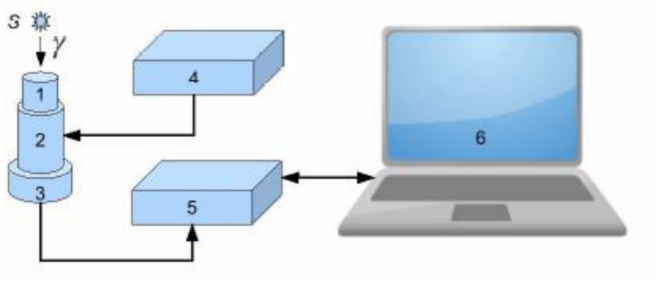
\includegraphics[width = 0.5\textwidth]{img/ust_labnik.png}
                \caption{Принципиальная блок-схема спектрометра. (1 – сцинтиллятор, 2 – ФЭУ, 3 – предусилитель импульсов, 4 – высоковольтный блок питания для ФЭУ, 5 – блок преобразования аналоговых импульсов с ФЭУ в цифровой код (АЦП), 6 – компьютер для сбора данных, их обработки и хранения).}
                \label{img:ust_labnik}
            \end{center}
        \end{figure}

        \begin{figure}[h!]
            \begin{center}
                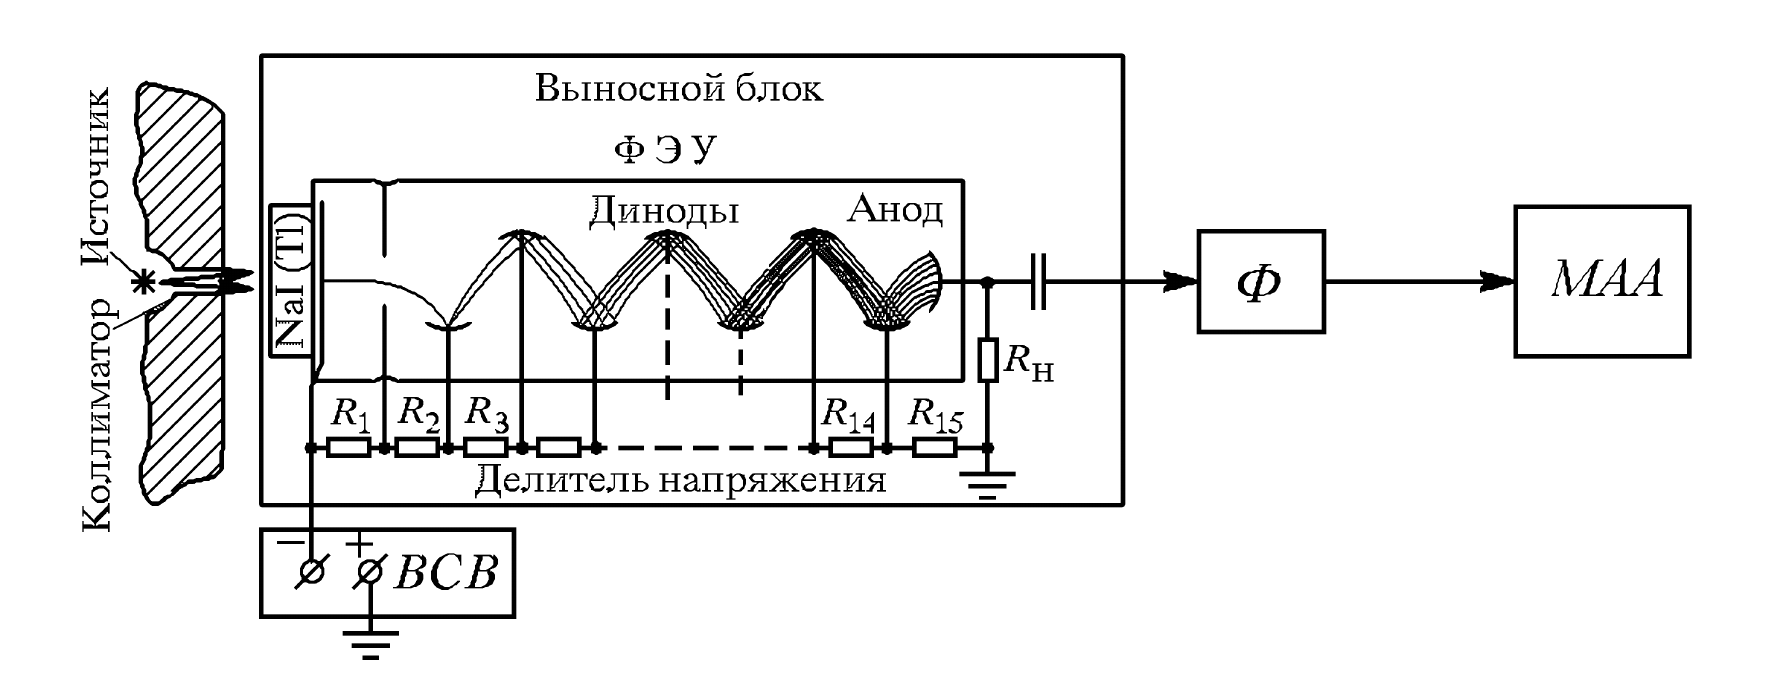
\includegraphics[width = 0.7\textwidth]{img/ust.png}
                \caption{Пример схематического устройства сцинтилляционного детектора}
                \label{img:ust}
            \end{center}
        \end{figure}

        Исследуемое излучение попадает на вещество-сцинтиллятор. Вещество представляет собой неорганический кристалл NaI(Tl). Для предотвращения сильного поглощения излучения в сцинтилляторе вводят небольшие добавки других атомов (в данном случае атомы Таллия). Свободные локальные уровни энергии электрона на примесных атомах таллия располагаются внутри запрещенной зоны кристалла NaI.
        В процессе релаксации возможны переходы электронов, возбужденных в зону проводимости, на эти уровни. Энергии излучаемых при таких переходах фотонов меньше ширины запрещенной зоны, и они могут поглощаться только атомами таллия. Но концентрация таллия мала (порядка $0,1\%$), поэтому мало поглощение указанных фотонов, и они имеют все шансы вылететь из сцинтиллятора. В этом случае прохождение ионизирующей частицы через вещество будет сопровождаться световой вспышкой, которая и может быть использована для регистрации частицы.

        Испущенный сцинтиллятором свет попадает на фотокатод и выбивает из него электроны, которые далее умножаются при помощи ФЭУ. На каждом уровне динодов один электрон выбивает несколько новых, образуя лавину. В конечном итоге электроны попадают на анод. При помощи предусилителя импульсов и АЦП сигнал регистрируется компьютером.

        \subsection{Энергетическое разрешение спектрометра}

            Даже при поглощении частиц с одинаковой энергией амплитуда импульса на выходе фотоприёмника сцинтилляционного детектора меняется от события к событию. Это связано:

            1)~со статистическим характером процессов сбора фотонов на фотоприёмнике и последующего усиления,
            2)~с различной вероятностью доставки фотона к фотоприёмнику из разных точек сцинтиллятора,
            3)~с разбросом высвечиваемого числа фотонов.

            В результате в экспериментальном спектре линия (которая для идеального детектора представляла бы дельта-функцию) оказывается размытой, её часто описывают гауссианом.

            Энергетическим разрешением спектрометра называется величина
            $$
                R_i = \frac{\Delta E_i}{E_i},
            $$
            где $\Delta E_i$ -- ширина пика полного поглощения, измеренная на половине высоты (в единицах энергии), $E_i$ -- энергия регистрируемых гамма-квантов. Значение $E_i$ пропорционально среднему числу фотонов $\bar{n_i}$ на входе ФЭУ:
            $$
                E \propto \bar{n}.
            $$

            Полуширина пика $\Delta E_i$ пропорциональна среднеквадратичной флуктуации $\bar{\Delta n_i}$. Так как $n_i$ распределено по закону Пуассона, то $\bar{\Delta n_i} = \sqrt{\bar{n_i}}$ и поэтому
            $$
                \Delta E_i \propto \sqrt{\bar{n_i}}.
            $$

            Из вышесказанного получаем:
            \begin{equation}
                R_i = \frac{\Delta E_i}{E_i} \propto \frac{1}{\sqrt{E_i}}.
                \label{eq:R}
            \end{equation}
            Таким образом, чем выше энергия гамма-кванта, тем меньше разрешение.

        \subsection{Форма импульсов}

            Схема ФЭУ представлена на рисунке \ref{img:FEU}

            \begin{figure}[h!]
                \begin{center}
                    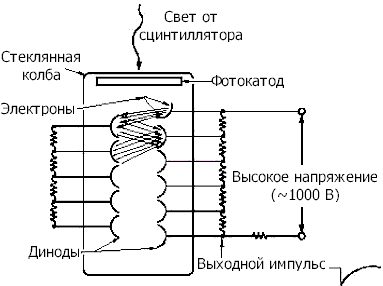
\includegraphics[width = 0.5\textwidth]{img/FEU.png}
                    \caption{Схема ФЭУ}
                    \label{img:FEU}
                \end{center}
            \end{figure}

            Сигнал на выходе имеет вид:
            $$
                U(t) \propto e^{-t/RC}(1 - e^{-t/\tau_0}
            $$
            где $\tau_0$ -- время высвечивания сцинтиллятора, а $RC$ -- постоянная времени, определяемая анодной цепью ФЭУ.

            Чтобы сигнал было удобно регистрировать, $RC$ выбирают много больше, чем $\tau_0$.

        \subsection{Спектры Co, Cs и Na}

            На рис. \ref{img:lab_co_cs}(a) изображён спектр излучения $^{60}Co$. На нём наблюдаются 2 фотопика (1) и (2) с энергиями $1.173 МэВ$ и $1.332 МэВ$. Также видим край комптоновского спектра (3), пик обратного рассеяния (4) и пик характеристического излучения свинца (5).

            На рис. \ref{img:lab_co_cs}(b) ($^{137}Cs$) видим фотопик (1) с энергией $0.6617 МэВ$, край комптоновского спектра (2) и пик обратного рассеяния (3).

            На рис. \ref{img:lab_na} ($^{22}Na$) наблюдается фотопик (1) с энергией $1.274 МэВ$, аннигиляционный пик (2) на $511 кэВ$, края комптоновских спектров (3) и (4), пик обратного рассеяния (5) и характеристическое излучение свинца (6).

            \begin{figure}[ht!]
                \centering
                \subfloat[\centering]{{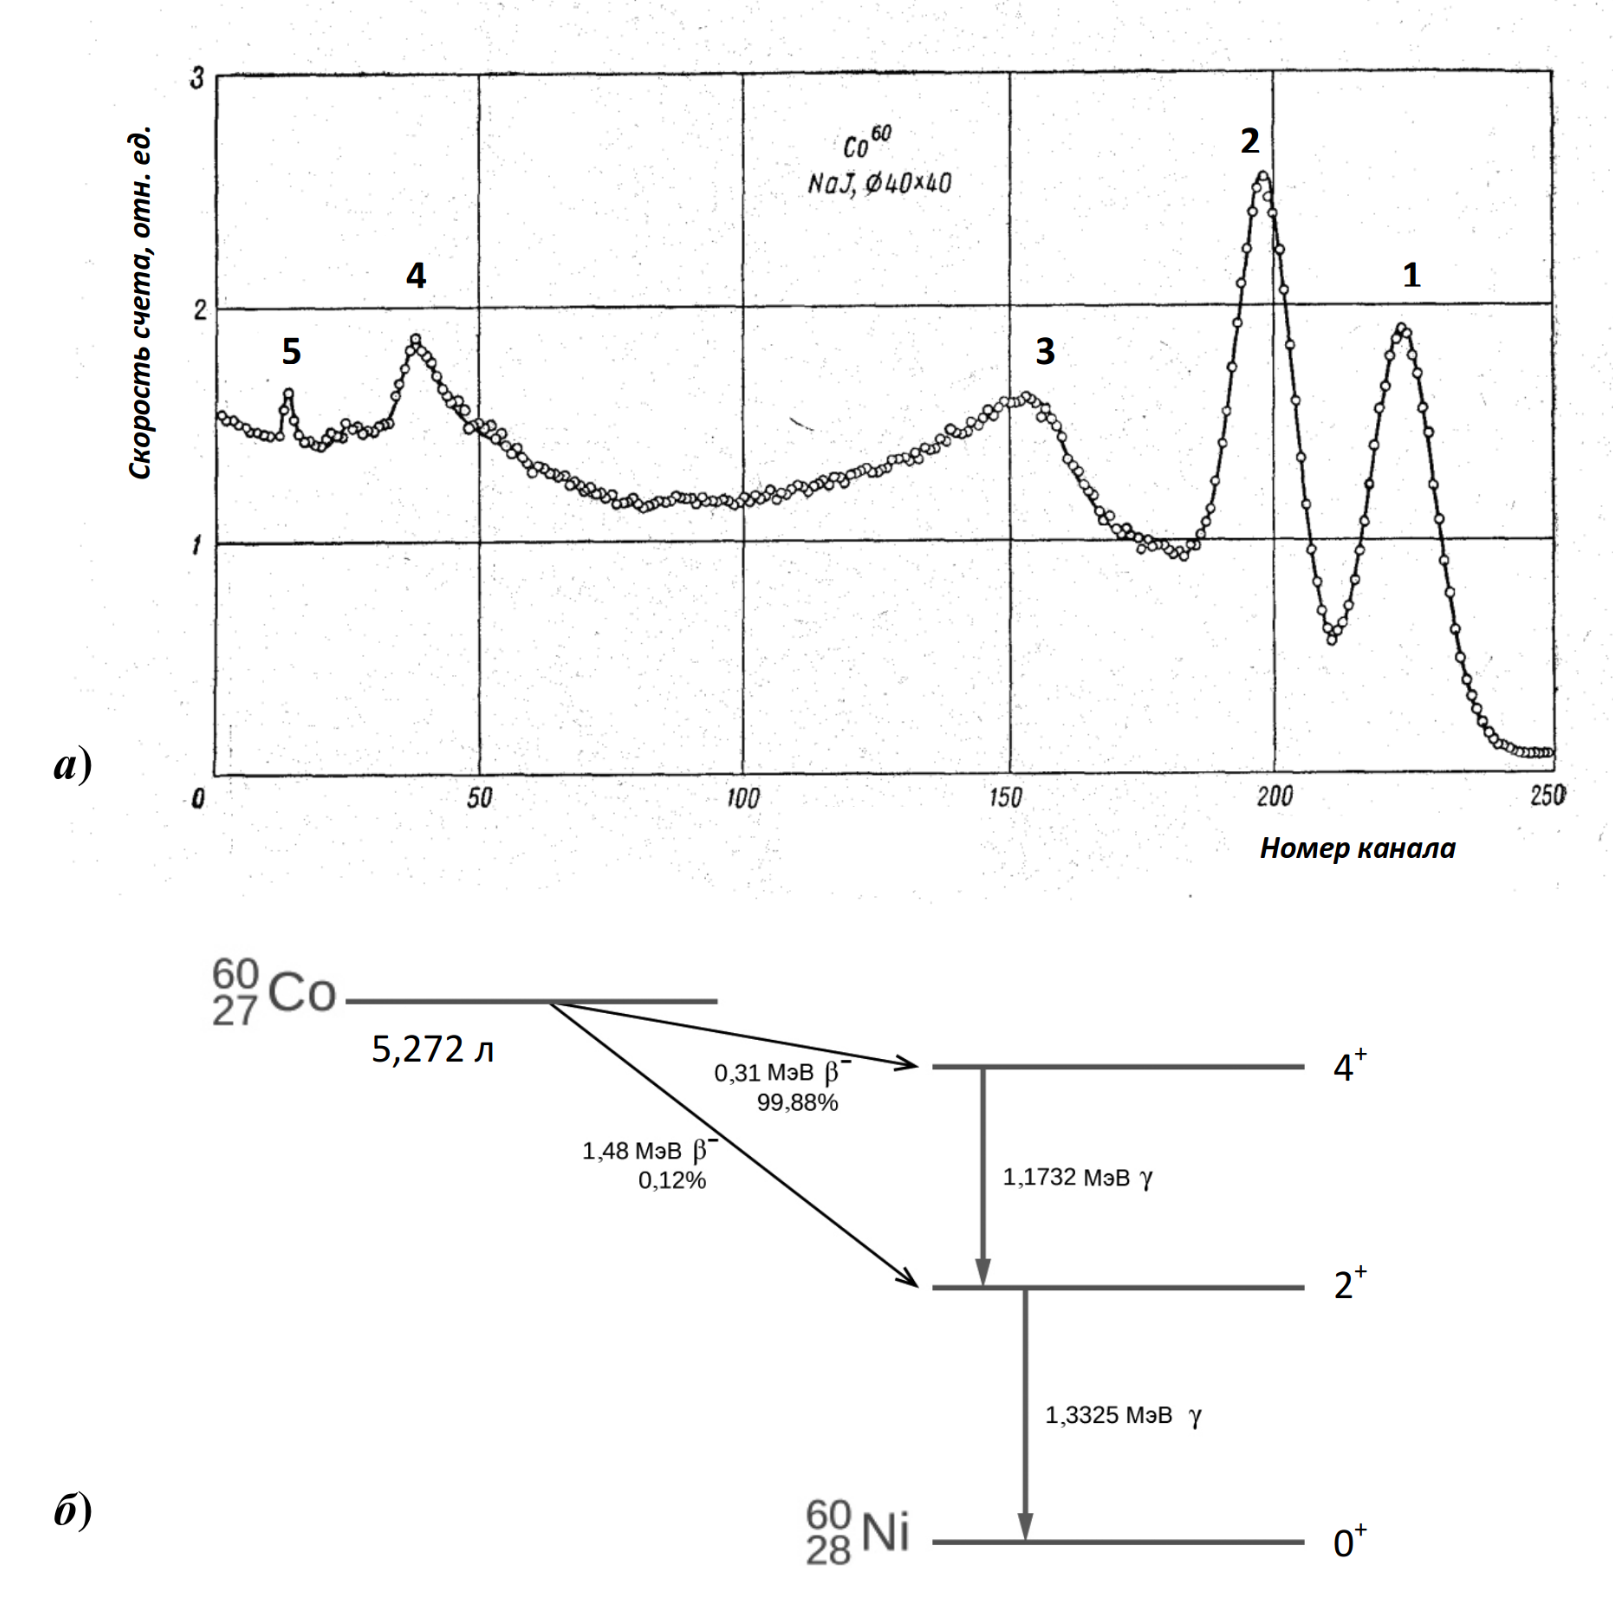
\includegraphics[width=0.4\linewidth]{img/lab_co.png}}}
                \qquad
                \subfloat[\centering]{{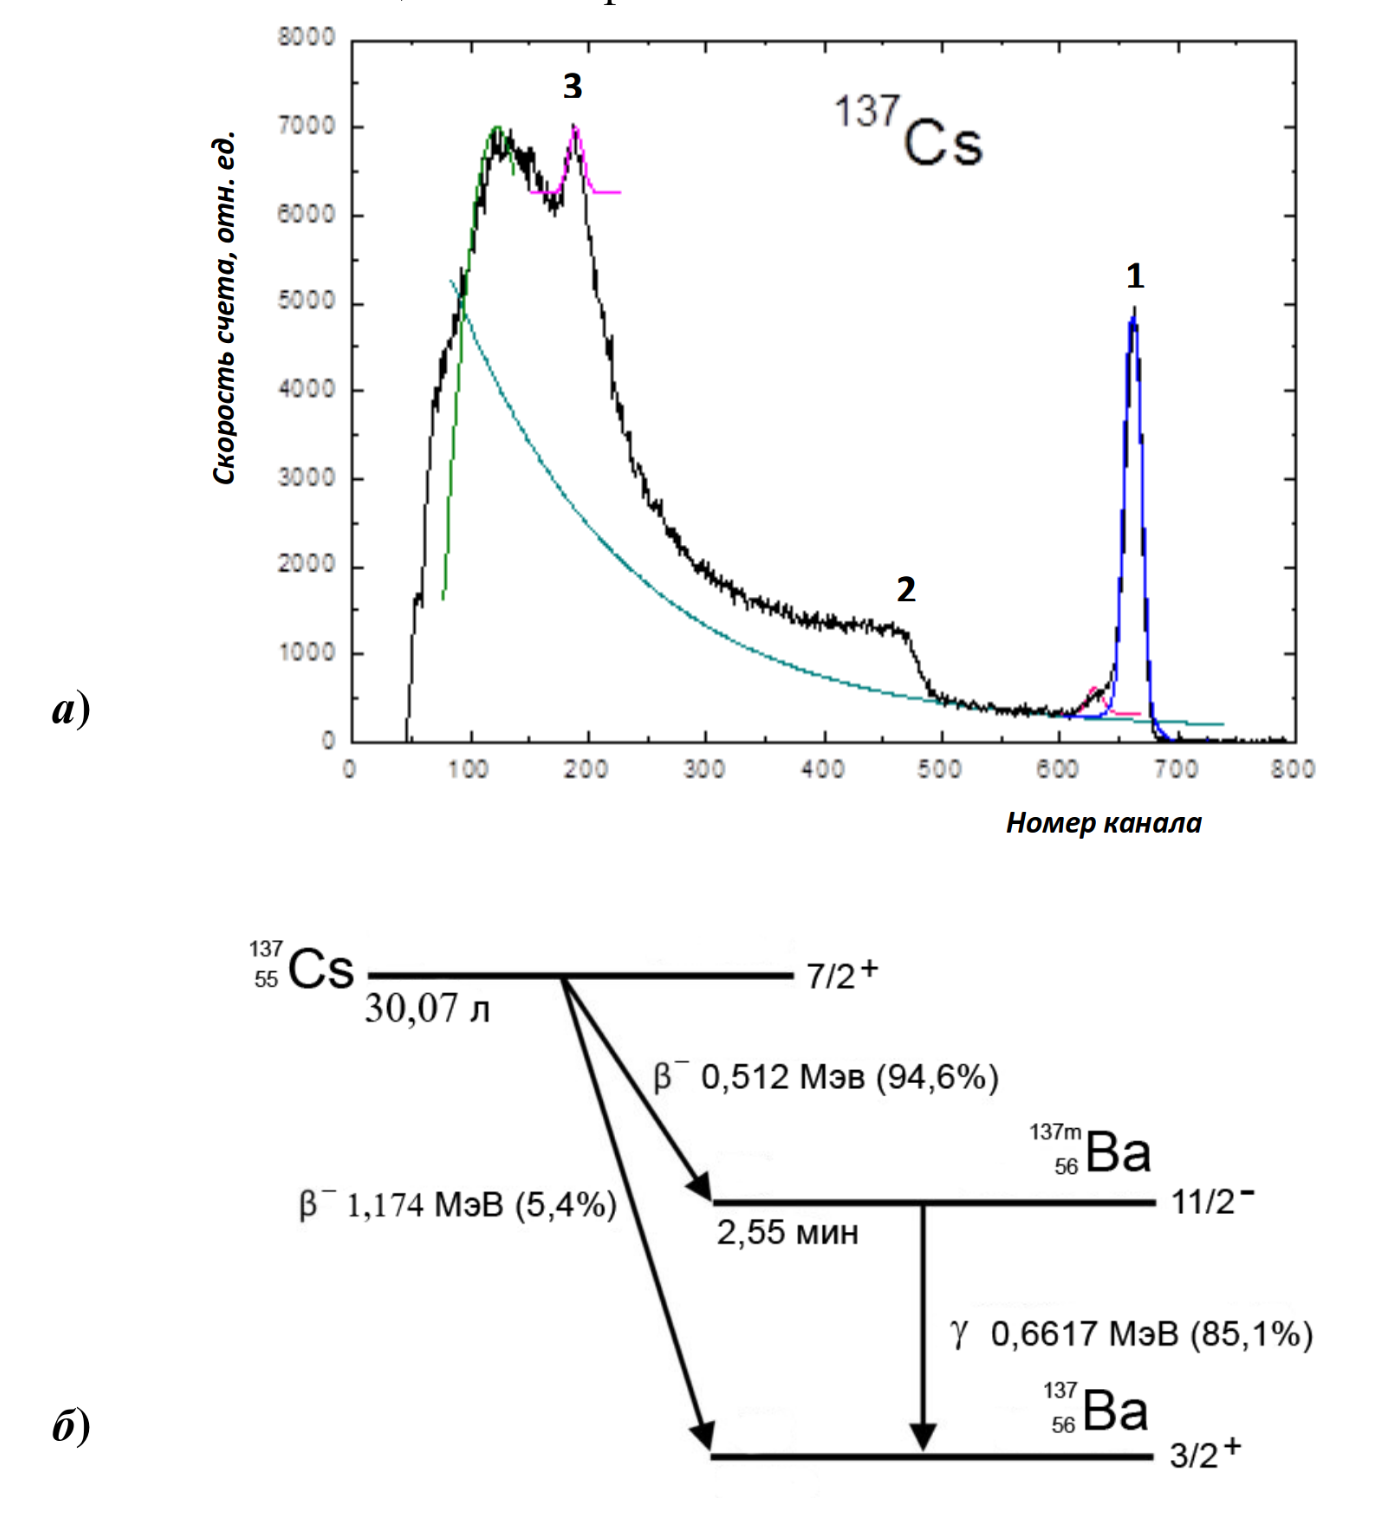
\includegraphics[width=0.4\linewidth]{img/lab_cs.png}}}
                \caption{Спектры для Co и Cs}%
                \label{img:lab_co_cs}%
            \end{figure}

            \begin{figure}[ht!]
                \begin{center}
                    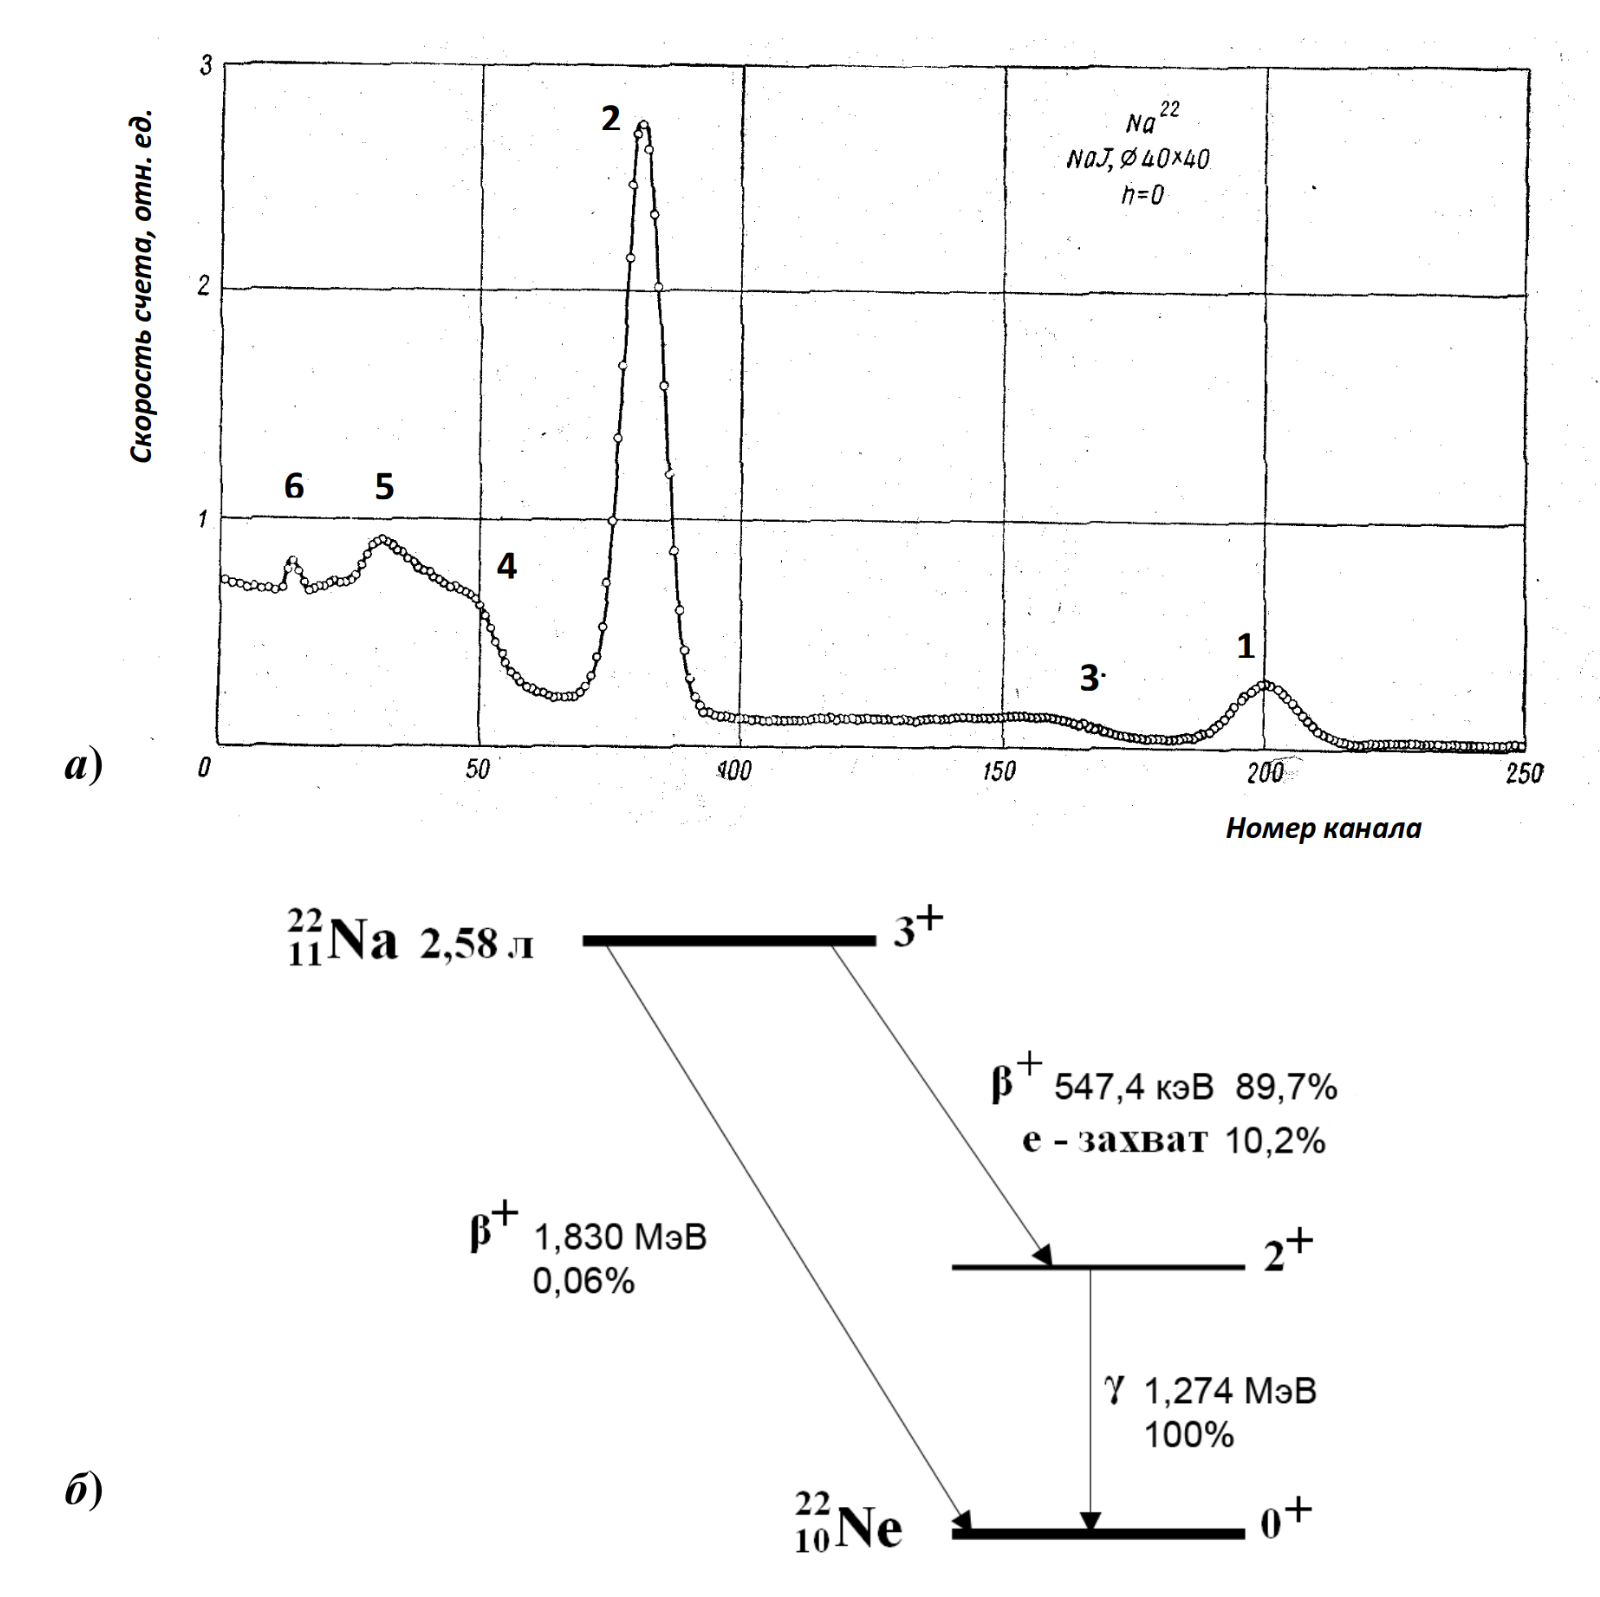
\includegraphics[width = 0.4\textwidth]{img/lab_na.png}
                    \caption{Спектр для Na}
                    \label{img:lab_na}
                \end{center}
            \end{figure}

    \section{Ход работы}

        Измерения для каждого источника проводились в течение 5 минут. Предварительно был измерен фон (рис. \ref{img:fon}).

        \begin{figure}[ht!]
            \begin{center}
                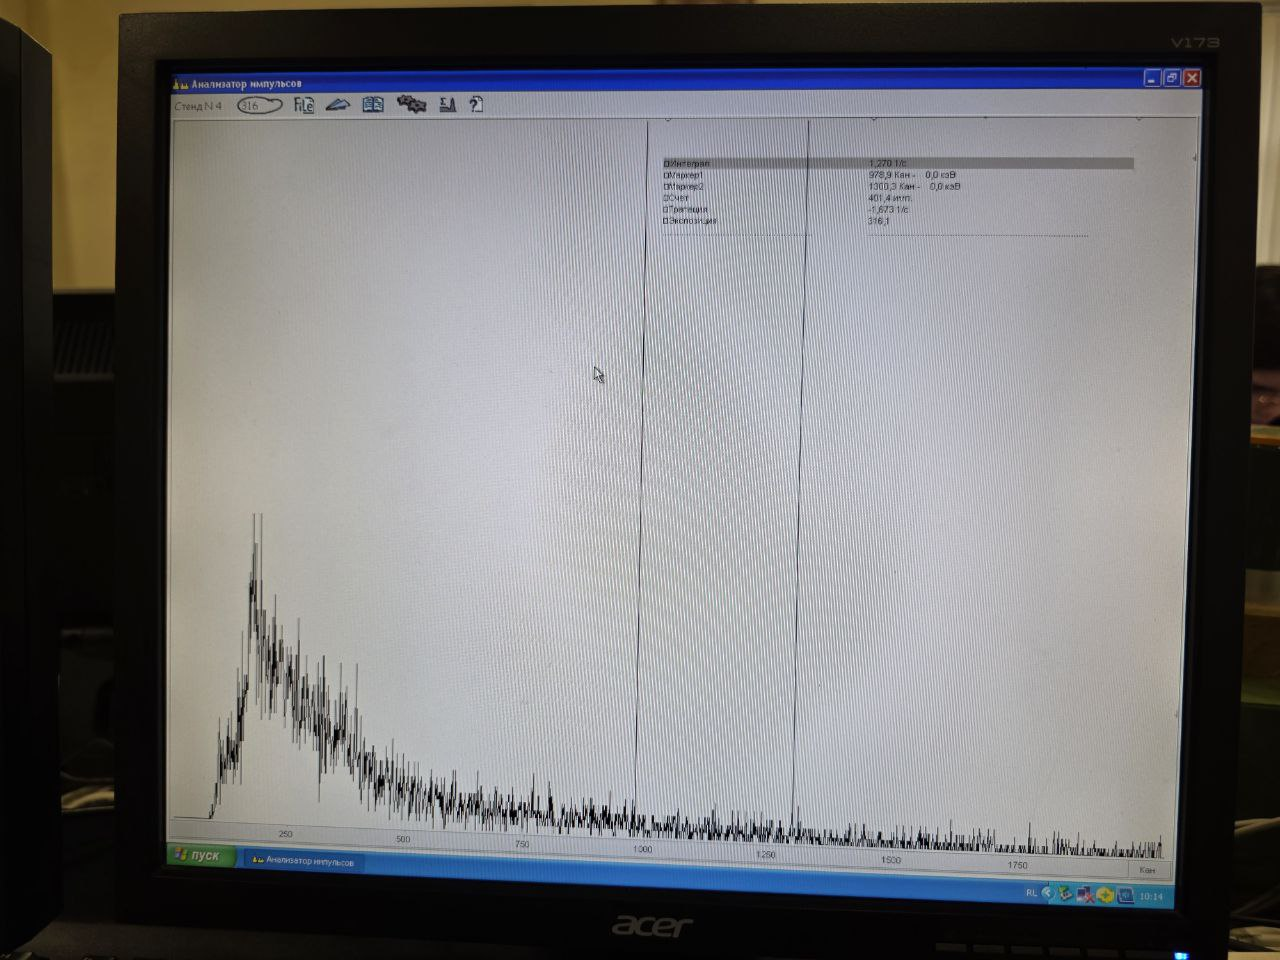
\includegraphics[width = 0.5\textwidth]{img/fon.jpg}
                \caption{Фоновый спектр}
                \label{img:fon}
            \end{center}
        \end{figure}

        \subsection{Калибровочный график}

            По пикам Co (рис. \ref{img:co_cs}(a)), Cs (рис. \ref{img:co_cs}(b)) и Na (рис. \ref{img:na}) проведём калибровочную прямую $N_i = kE_i + b$ для нахождения соответствия между энергиями и номерами каналов спектрометра. Полученная прямая на рис. \ref{plot:calibration}.
            Значения $k$ и $b$:

            \begin{align*}
                k &= 1360 \pm 10 & b &= 74 \pm 10
            \end{align*}

            \begin{figure}[ht!]
                \begin{center}
                    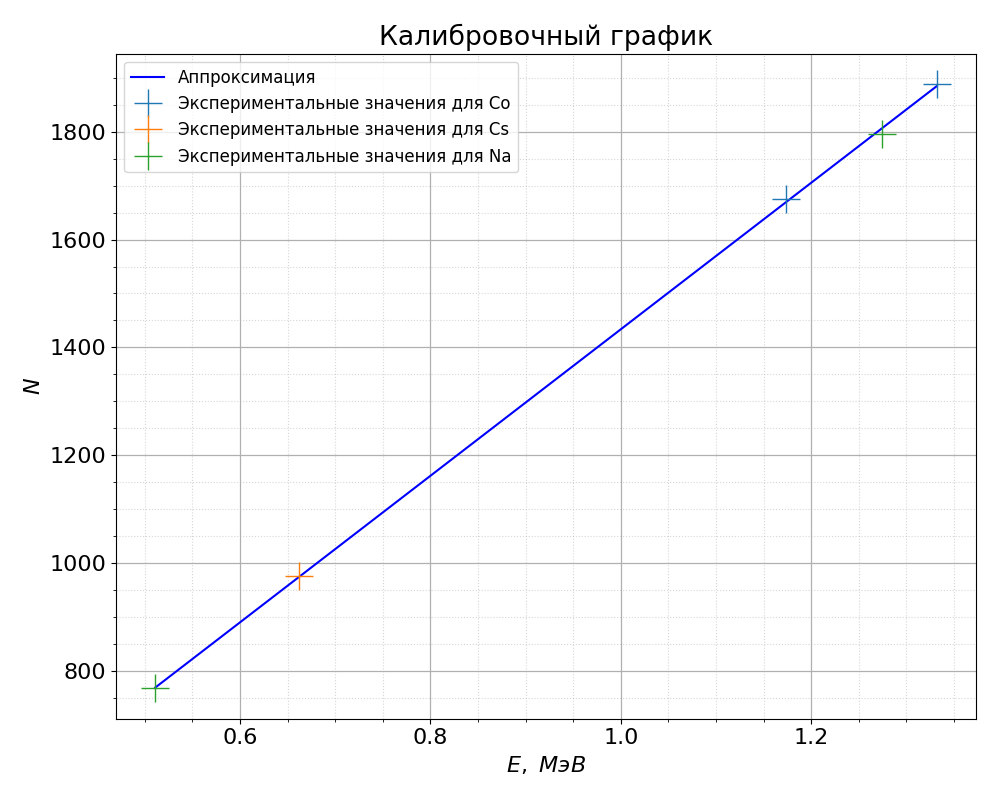
\includegraphics[width = 0.5\textwidth]{img/calibration.png}
                    \caption{Калибровочный график}
                    \label{plot:calibration}
                \end{center}
            \end{figure}

            Расчётные формулы:

            \begin{align*}
                E_i &= \frac{N_i - b}{k} & \sigma_{E_i} &= \sqrt{\left( \frac{-1}{k} \right)^2 \sigma_b^2 + \left( \frac{b - N_i}{k^2} \right)^2 \sigma_k^2}
            \end{align*}

            \begin{align*}
                \Delta E_i &= \frac{\Delta N_i}{k} & \sigma_{\Delta E_i} &= \frac{\Delta N_i}{k^2} \sigma_k
            \end{align*}

            \begin{align*}
                R_i &= \frac{\Delta E_i}{E_i} & \sigma_{R_i} &= \sqrt{\left( \frac{1}{E_i} \right)^2 \sigma_{\Delta E_i}^2 + \left( \frac{-\Delta E_i}{E_i^2} \right)^2 \sigma_{E_i}^2}
            \end{align*}

            Результаты для кобальта, цезия и натрия в таблице \ref{tab:cal_res}.

            \begin{table}[!ht]
                \centering
                \begin{tabular}{|c|c|c|c|c|c|c|}
                    \hline

                    Источник & $N_i$ & $\Delta N_i$ & $E_{i_{таб}}, кэВ$ & $E_i, кэВ$ & $\Delta E_i, кэВ$ & $R_i$\\ \hline
                    Co & $1675$ & $76$ & $1173$ & $1180 \pm 10$ & $55.9 \pm 0.8$ & $0.0475 \pm 0.0007$\\ \hline
                    Co & $1889$ & $96$ & $1332$ & $1330 \pm 10$ & $70.6 \pm 0.9$ & $0.0529 \pm 0.0007$\\ \hline
                    Cs & $975$ & $60$ & $661.7$ & $663 \pm 9$ & $44.1 \pm 0.8$ & $0.0666 \pm 0.0012$\\ \hline
                    Na & $767$ & $54$ & $511$ & $510 \pm 8$ & $39.7 \pm 0.8$ & $0.078 \pm 0.002$\\ \hline
                    Na & $1796$ & $128$ & $1274$ & $1270 \pm 10$ & $94.14 \pm 1.00$ & $0.0743 \pm 0.0008$\\ \hline

                \end{tabular}
                \caption{Таблица измерений для Co, Cs и Na}
                \label{tab:cal_res}
            \end{table}

        \subsection{Результаты измерений для Am и Eu}

            Измерения америция и европия на рис. \ref{img:am_eu}.

            Результаты в таблице \ref{tab:am_eu_res}. Для Европия отчётливо наблюдаются пики обратного рассеяния и пики, полученные в результате сложения нескольких $\gamma$-квантов (при попадании нескольких $\gamma$-квантов за время одного счёта детектора).

            \begin{table}[!ht]
                \centering
                \begin{tabular}{|c|c|c|c|c|c|}
                    \hline

                    Источник & $N_i$ & $\Delta N_i$ & $E_i, кэВ$ & $\Delta E_i, кэВ$ & $R_i$\\ \hline
                    Am & $99$ & $11$ & $18 \pm 8$ & $8.1 \pm 0.7$ & $0.44 \pm 0.07$\\ \hline
                    Am & $150$ & $16$ & $56 \pm 8$ & $11.8 \pm 0.7$ & $0.21 \pm 0.01$\\ \hline
                    Eu & $118$ & $16$ & $32 \pm 8$ & $11.8 \pm 0.7$ & $0.36 \pm 0.03$\\ \hline
                    Eu (+) & $169$ & $8$ & $70 \pm 8$ & $5.9 \pm 0.7$ & $0.084 \pm 0.011$\\ \hline
                    Eu (r) & $188$ & $15$ & $84 \pm 8$ & $11.0 \pm 0.7$ & $0.131 \pm 0.009$\\ \hline
                    Eu & $236$ & $17$ & $119 \pm 8$ & $12.5 \pm 0.7$ & $0.105 \pm 0.006$\\ \hline
                    Eu (r) & $298$ & $20$ & $165 \pm 8$ & $14.7 \pm 0.7$ & $0.089 \pm 0.005$\\ \hline
                    Eu (+) & $401$ & $30$ & $241 \pm 8$ & $22.1 \pm 0.8$ & $0.092 \pm 0.003$\\ \hline
                    Eu & $537$ & $41$ & $341 \pm 8$ & $30.2 \pm 0.8$ & $0.089 \pm 0.002$\\ \hline
                    Eu (+) & $650$ & $80$ & $424 \pm 8$ & $58.8 \pm 0.8$ & $0.139 \pm 0.002$\\ \hline
                    Eu (+) & $1135$ & $72$ & $780 \pm 9$ & $53.0 \pm 0.8$ & $0.0679 \pm 0.0011$\\ \hline
                    Eu (+) & $1384$ & $86$ & $964 \pm 10$ & $63.3 \pm 0.9$ & $0.0656 \pm 0.0009$\\ \hline
                    Eu (+) & $1582$ & $91$ & $1109 \pm 11$ & $66.9 \pm 0.9$ & $0.0603 \pm 0.0008$\\ \hline

                \end{tabular}
                \caption{Результаты измерений для Америция и Европия. (r) - пик обратного рассеяния; (+) - пик, полученный в результате "почти одновременного" попадания $\gamma$-квантов более низких энергий в детектор (сложение)}
                \label{tab:am_eu_res}
            \end{table}

        \subsection{Край комптоновского поглощения}

            Построим график, по одной оси которого измеренные значения края комптоновского поглощения, а по другой теоретические. Результаты в таблице \ref{tab:compton} и на рис. \ref{plot:compton}. Расчётные формулы:

            \begin{align*}
                E_c &= \frac{\hbar \omega}{1 + \frac{mc^2}{2 \hbar \omega}} & \sigma_{E_c} &= 4 \hbar \omega \frac{mc^2 + \hbar \omega}{(mc^2 + 2\hbar \omega)^2} \sigma_{\hbar \omega}
            \end{align*}

            \begin{figure}[ht!]
                \begin{center}
                    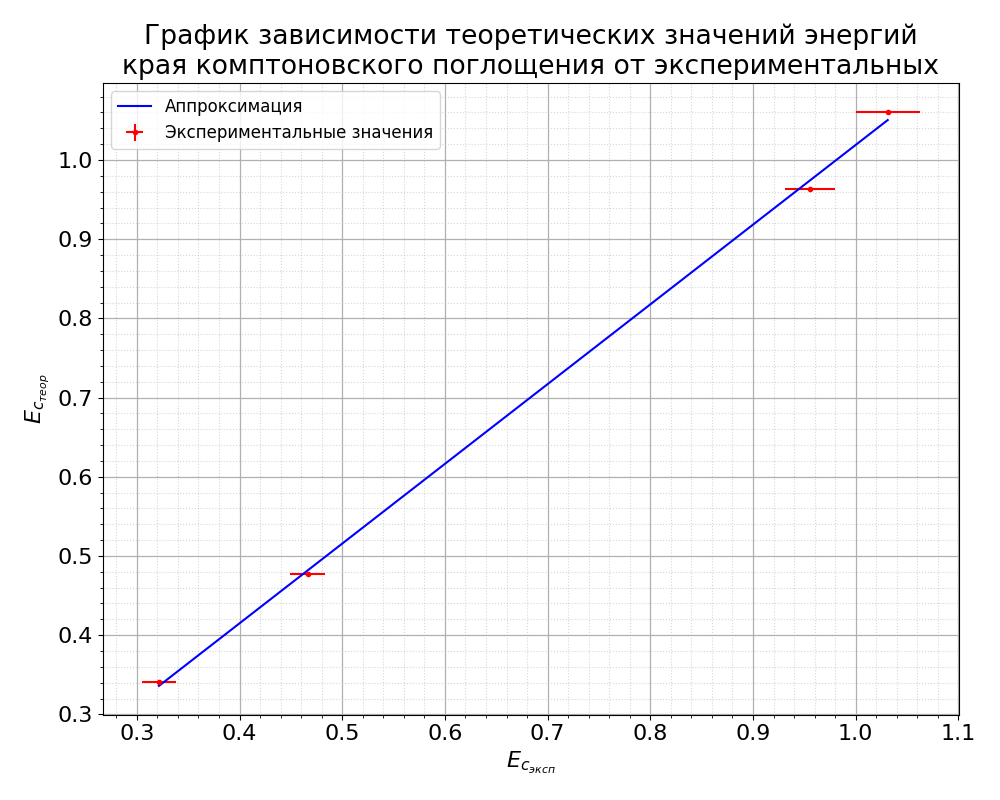
\includegraphics[width = 0.5\textwidth]{img/compton.png}
                    \caption{График зависимости теоретических значений энергий края комптоновского поглощения от экспериментальных}
                    \label{plot:compton}
                \end{center}
            \end{figure}

            \begin{table}[!ht]
                \centering
                \begin{tabular}{|c|c|c|}
                    \hline

                    Источник & $E_{c_{эксп}}$ & $E_{c_{теор}}$\\ \hline
                    Co & -- & $1.12$\\ \hline
                    Co & $0.96 \pm 0.02$ & $0.963$\\ \hline
                    Cs & $0.47 \pm 0.02$ & $0.477$\\ \hline
                    Na & $1.03 \pm 0.03$ & $1.06$\\ \hline
                    Na & $0.32 \pm 0.02$ & $0.341$\\ \hline

                \end{tabular}
                \caption{Экспериментальные и теоретические значения энергий края комптоновского поглощения}
                \label{tab:compton}
            \end{table}

        \subsection{Проверка зависимости (\ref{eq:R})}

            Построим график $R_i^2 = f(1/E_i)$. Значения для америция, а также первый фотопик европия исключим из-за больших погрешностей. График на рисунке \ref{plot:check_r}

            \begin{figure}[ht!]
                \begin{center}
                    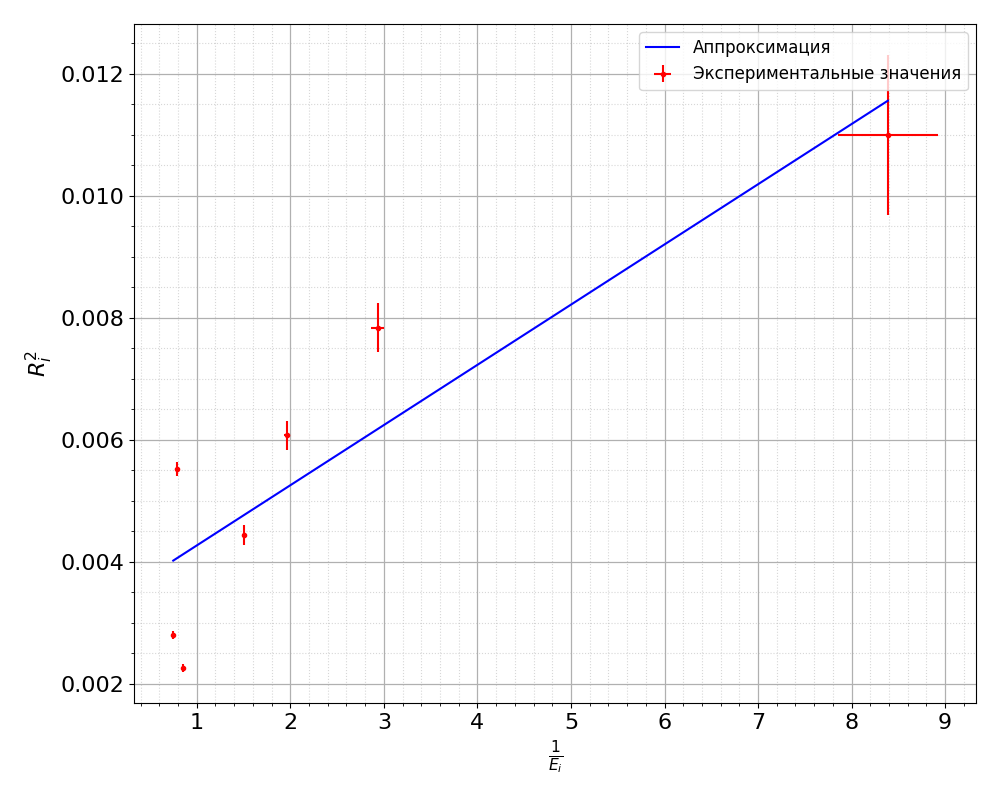
\includegraphics[width = 0.5\textwidth]{img/plot_r.png}
                    \caption{График для проверки зависимости $R_i \propto \frac{1}{\sqrt{E_i}}$}
                    \label{plot:check_r}
                \end{center}
            \end{figure}

            Как видим, пронаблюдать подтверждение зависимости не удалось. Скорее всего, имеет место слишком неточное измерение ширины на полувысоте пиков.

        \subsection{Пики обратного рассеяния}

            Рассчитаем значения энергии пиков обратного рассеяния по формуле:

            \begin{align*}
                E_{обр} &= \frac{E}{1 + 2E/mc^2} & \sigma_{E_{обр}} &= \frac{(mc^2)^2}{mc^2 + 2E} \sigma_E
            \end{align*}

            Результаты в таблице \ref{tab:check_r} и на рисунке \ref{plot:check_r}.

            \begin{table}[!ht]
                \centering
                \begin{tabular}{|c|c|c|c|}
                    \hline

                    Источник & $E, МэВ$ & $E_{обр_{теор}}, МэВ$ & $E_{обр_{эксп}}, МэВ$\\ \hline
                    Co & $1.178 \pm 0.011$ & $0.2099 \pm 0.0004$ & -- \\ \hline
                    Co & $1.335 \pm 0.012$ & $0.2145 \pm 0.0003$ & $0.22 \pm 0.02$ \\ \hline
                    Cs & $0.663 \pm 0.009$ & $0.1844 \pm 0.0007$ & $0.18 \pm 0.02$\\ \hline
                    Na & $0.510 \pm 0.008$ & $0.1702 \pm 0.0009$ & $0.17 \pm 0.02$\\ \hline
                    Na & $1.267 \pm 0.012$ & $0.2126 \pm 0.0003$ & -- \\ \hline
                    Am & $0.056 \pm 0.008$ & $0.046 \pm 0.005$ & -- \\ \hline
                    Eu & $0.341 \pm 0.008$ & $0.146 \pm 0.001$ & $0.165 \pm 0.008$ \\ \hline
                    Eu & $0.119 \pm 0.008$ & $0.081 \pm 0.004$ & $0.084 \pm 0.008$ \\ \hline
                    Eu & $0.032 \pm 0.008$ & $0.029 \pm 0.006$ & -- \\ \hline

                \end{tabular}
                \caption{Значения энергий пиков обратного рассеяния}
                \label{tab:check_r}
            \end{table}

            \begin{figure}[ht!]
                \begin{center}
                    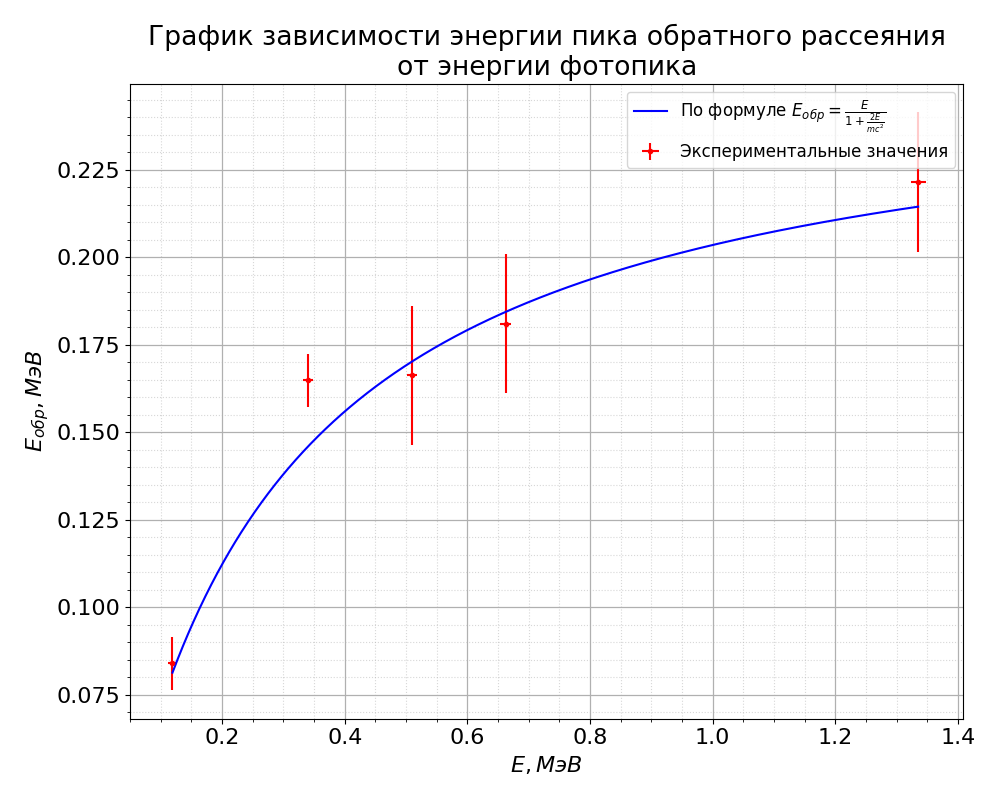
\includegraphics[width = 0.5\textwidth]{img/plot_rev.png}
                    \caption{График для проверки зависимости энергии пиков обратного рассеяния от энергии фотопиков}
                    \label{plot:check_r}
                \end{center}
            \end{figure}

        \subsection{Характеристическое излучение свинца}

            Заметим, что на графиках натрия, цезия и кобальта в левой части спектра наблюдается пик, соответствующий энергии порядка $90 кэВ$. Это соответствует характеристическому излучению из свинца, служащего защитой спектрометра от внешнего излучения.

    \section{Вывод}

        В ходе работы исследовали явления фотоэффекта, комптоновского рассеяния, образования электрон-позитронных пар и обратного рассеяния.

    \section{Необработанные измерения}

        \begin{figure}[ht!]
            \centering
            \subfloat[\centering]{{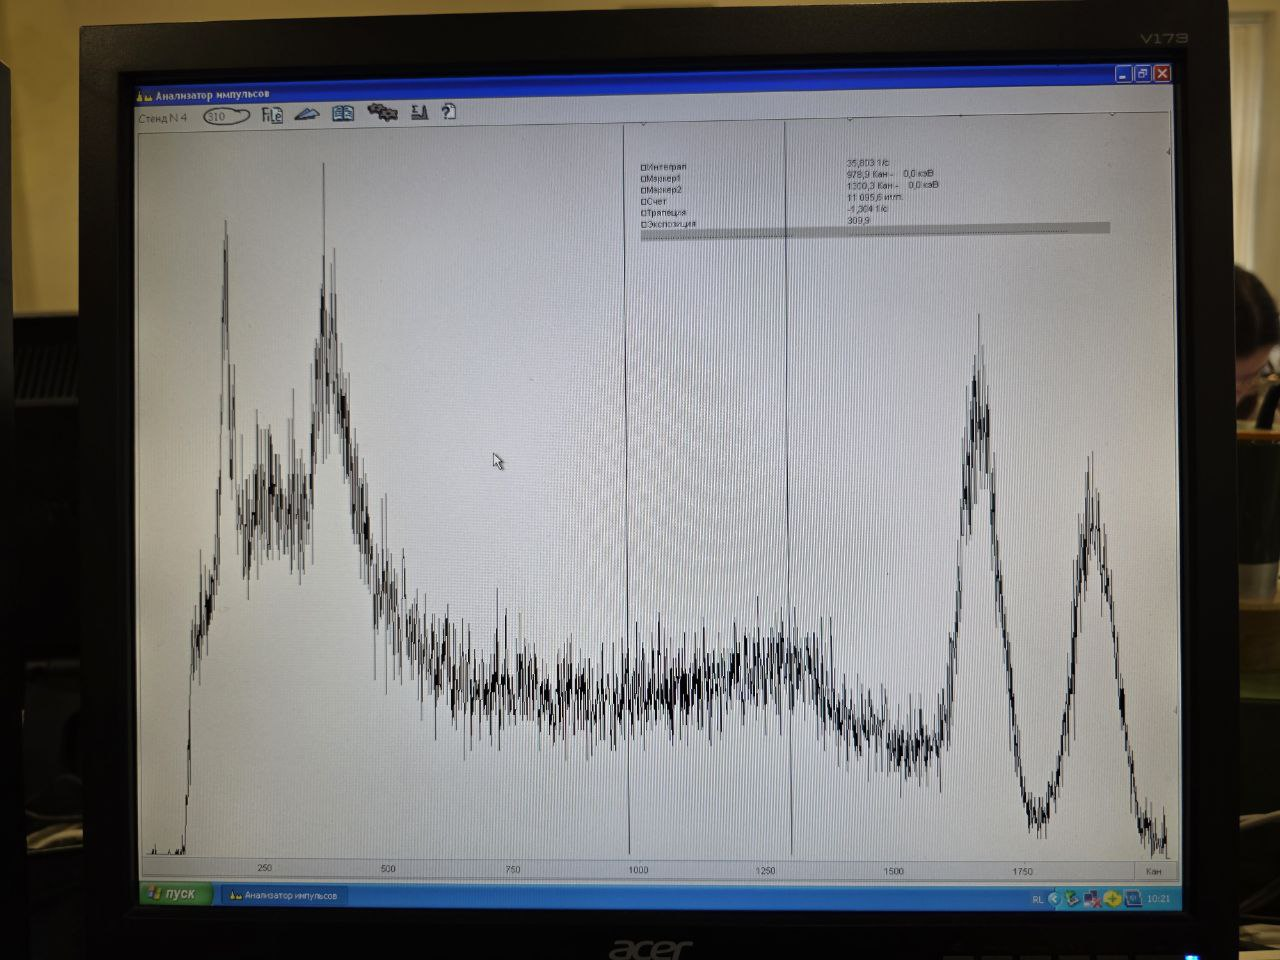
\includegraphics[width=0.45\linewidth]{img/co.jpg}}}
            \qquad
            \subfloat[\centering]{{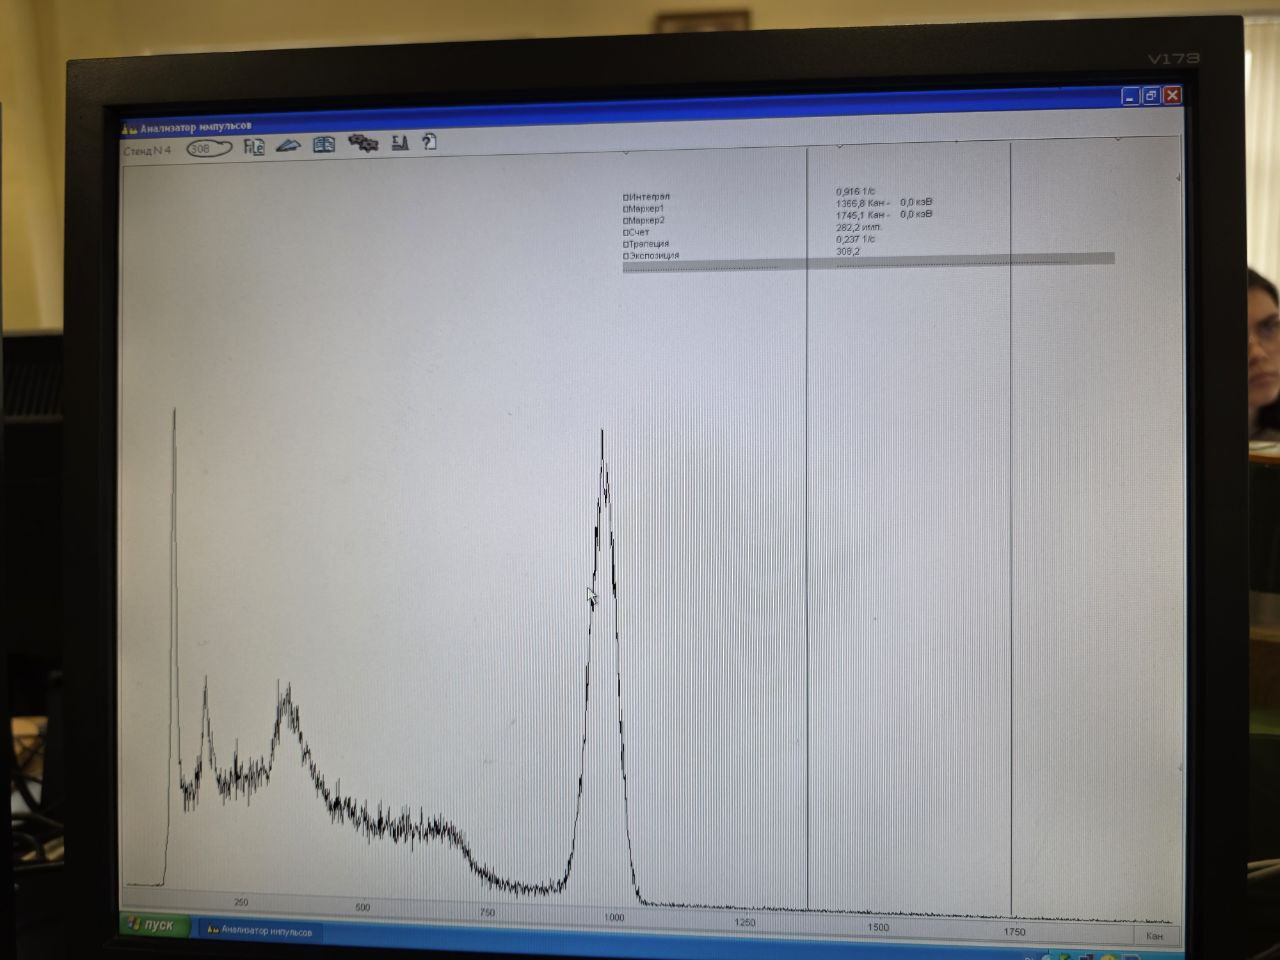
\includegraphics[width=0.45\linewidth]{img/cs.jpg}}}
            \caption{Измерения для Co и Cs}%
            \label{img:co_cs}%
        \end{figure}

        \begin{figure}[ht!]
            \begin{center}
                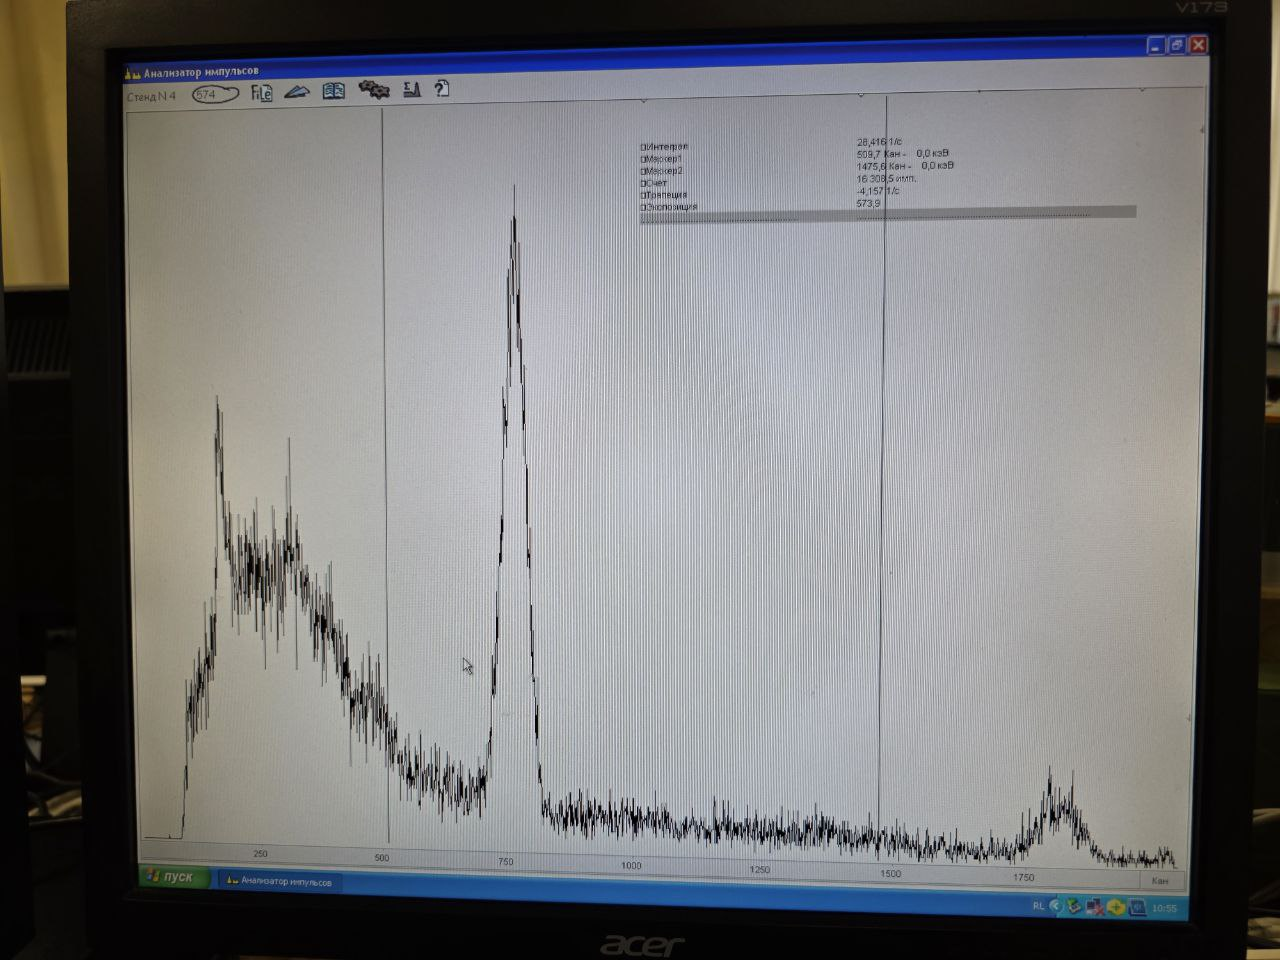
\includegraphics[width = 0.45\textwidth]{img/na.jpg}
                \caption{Измерения для Na}
                \label{img:na}
            \end{center}
        \end{figure}

        \begin{figure}[ht!]
            \centering
            \subfloat[\centering]{{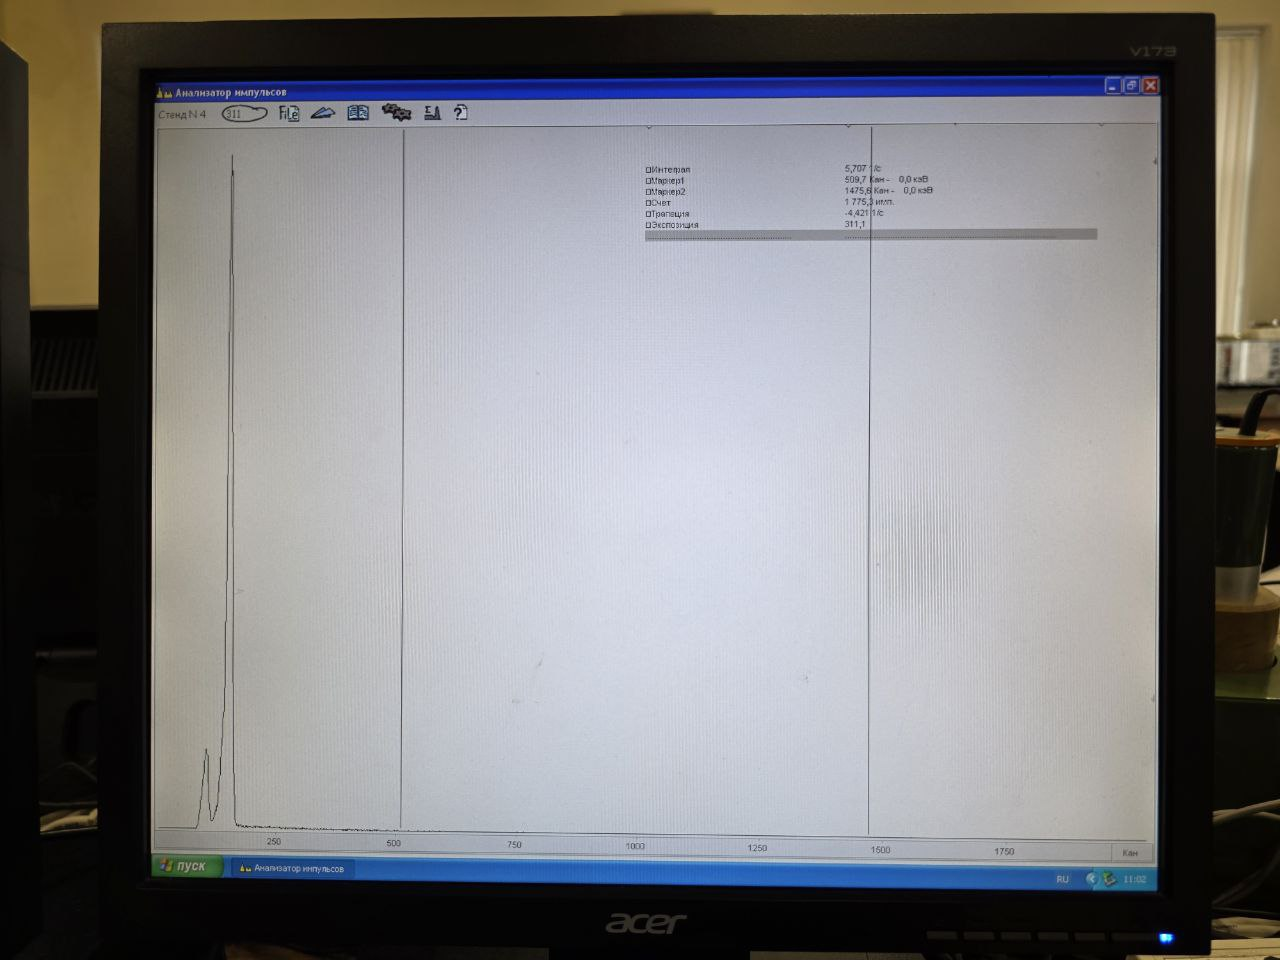
\includegraphics[width=0.45\linewidth]{img/am.jpg}}}
            \qquad
            \subfloat[\centering]{{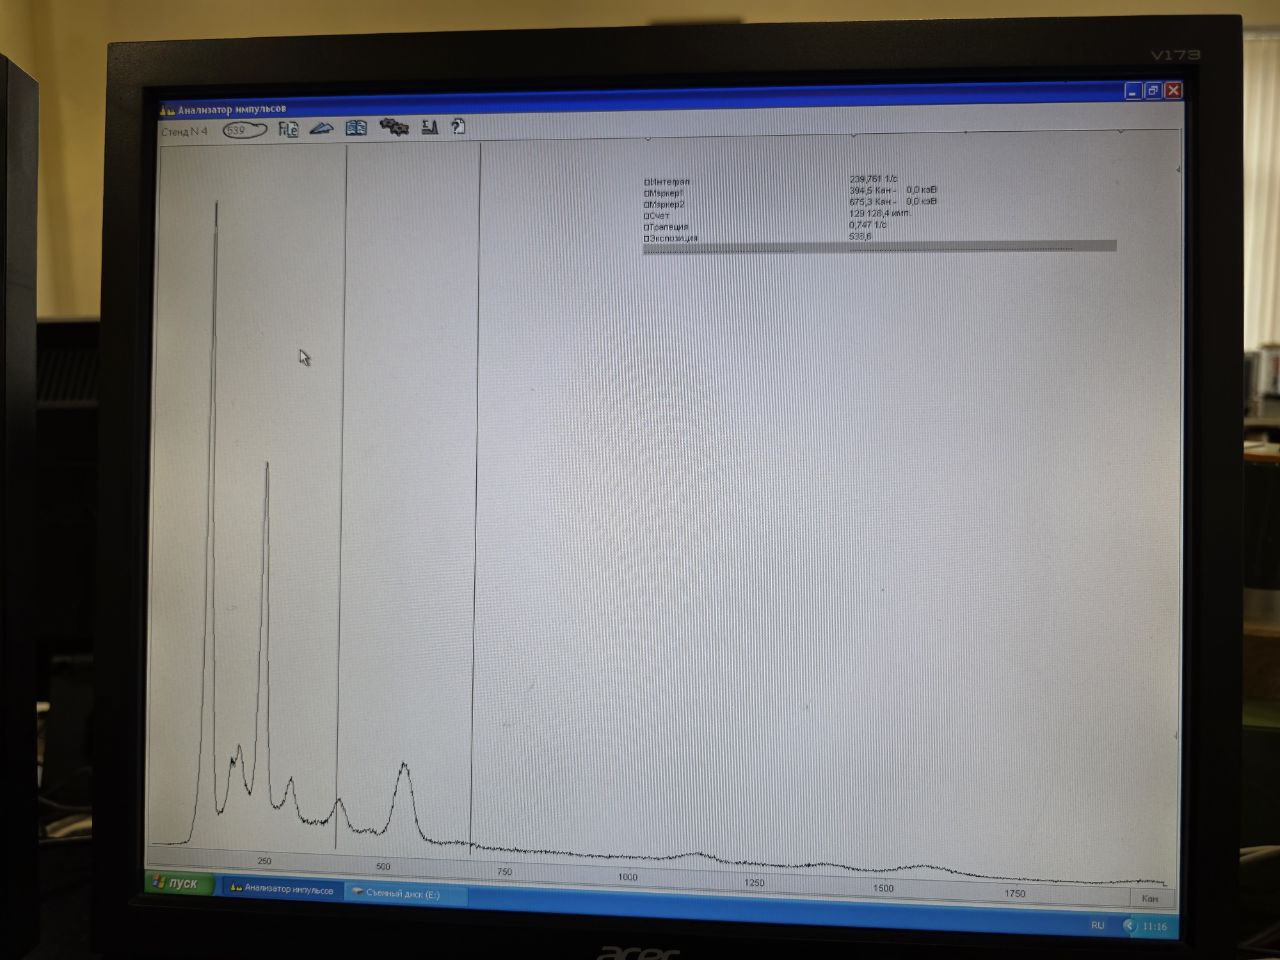
\includegraphics[width=0.45\linewidth]{img/eu.jpg}}}
            \caption{Измерения для Am и Eu}%
            \label{img:am_eu}%
        \end{figure}



\end{document}
